\documentclass[10pt,twocolumn]{article}

% use the oxycomps style file
\usepackage{oxycomps}

% usage: \fixme[comments describing issue]{text to be fixed}
% define \fixme as not doing anything special
\newcommand{\fixme}[2][]{#2}
% overwrite it so it shows up as red
\renewcommand{\fixme}[2][]{\textcolor{red}{#2}}
% overwrite it again so related text shows as footnotes
%\renewcommand{\fixme}[2][]{\textcolor{red}{#2\footnote{#1}}}
\usepackage{graphicx} % Required for \rotatebox
\usepackage{makecell} % Required for \makecell
% read references.bib for the bibtex data
\bibliography{references}

% include metadata in the generated pdf file
\pdfinfo{
    /Title (Integrating Feature Extraction with CNN using Dermoscopic images for enhanced melanoma detection)
    /Author (Joshua Wong)
}

% set the title and author information
\title{Integrating Feature Extraction with CNN using Dermoscopic images for enhanced melanoma detection
}
\author{Joshua Wong}
\affiliation{Occidental College}
\email{jwong5@oxy.edu}

\begin{document}

\maketitle
\footnote{https://www.overleaf.com/read/xffjtvvtvhtz}

\section{Introduction and Problem Context}

According to the American Academy of Dermatology Association, skin cancer is one of the most common cancers in the United States with approximately 9500 new cases every day and more than two people die every hour and according to the Skin Cancer Foundation, the annual cost of treating skin cancers is about 8.1 billions dollars \cite{AmericanAcademy}.
\newline
\newline
Melanoma is one of the deadliest skin cancers and is responsible for more than 70\% of all skin cancer related deaths. According to World Cancer Research Fund International, there were 324,635 cases of melanoma diagnosed worldwide and in 2020; the global death from melanoma was 57,043. As deadly as it is, the 5 year survival rate of melanoma is 99\% if detected early \cite{MelanomaIntro}. However, a significant challenge in patient care in the United States is the extended wait time for dermatology consultations, averaging 32 days \cite{Alexander} and the cost will be around 150-350 USD per visit, of which many patients may not be able to afford \cite{MiiSkin_2023}.
\newline
\newline
Dermoscopy has been shown to be very useful in differentiating melanocytic and non melanocytic lesions. Many primary care practitioners using the technique found that they have less referral to dermatologists which will cut the patients’ cost and time. Proficiency in the technique will also cut down on unnecessary biopsies and therefore less cost and suffering for patients. 
\newline
\newline
There have been numerous studies showing that artificial intelligence can be just as good or even better than dermatologists’ in diagnosing skin lesions. In the Pham et al. study, a deep-CNN architecture was tested in binary classification against dermatologists’ performances; it was shown that AI resulted in an AUC of 94.4\% which is 27.3\% better than the average of dermatologists and 23.3\% better than general practitioners. Furthermore, Pham’s AI model achieved much higher sensitivity and specificity, calculated 0.85 and 0.95 compared to 0.74 and 0.60 by dermatologists \cite{pham2021ai}.
\newline
\newline
In view of the usefulness of the AI dermoscopic diagnosis, many technological companies have developed applications capable of analyzing skin or lesions. These apps are now available in primary care practitioners’ and dermatologists’ offices to assist clinicians in diagnosing skin lesions. People can also download dermoscopic apps in their mobile phones if they want to find out whether their skin lesions are suspicious before seeing their doctors. 
\newline
\newline
The objective of this project is to design an advanced machine learning model, utilizing Convolutional Neural Networks (CNN) and feature extraction techniques. This model aims to achieve optimal diagnostic accuracy in identifying specific structures and patterns between melanoma and melanocytic nevus. Hopefully, it will eventually lead to improvements in diagnostic algorithms in skin lesions detection.
\newline
\newline
A long term objective of research in using AI in dermoscopic imaging is to be able to attract more interest of both primary care practitioners and specialists in AI dermoscopy platforms. The Polesie et al study in 2020 found that while 85\% of dermatologists were aware of AI as an emerging field, only 24\% reported good or excellent knowledge on the subject \cite{stiff2022artificial}. It is hoped that when the use of AI imaging becomes more popular, more dermatologists and primary care practitioners will be using AI assisted dermoscopy to improve diagnostic accuracy and detect skin cancers at their earliest stages. Besides the possibility of saving lives, AI dermoscopy can also decrease unnecessary biopsies or referrals; hence, saving patients’ money and time. 
\newline
\section{Technical Background}
\subsection{Dermatology}
Dermoscopy is a non-invasive imaging technique to examine skin lesions by illuminating and magnifying the surface of the skin. Under the dermoscope, blood vessels will be red and collagen will be white and structures such as networks and granules will be visible. The depth of the melanocytic lesion will reveal a different color as it will be black superficially in the stratum corneum, brown in the epidermis and blue in the deeper dermis \cite{sonthalia2019dermoscopy}. In 2002, Bafounta et al found that Dermoscopy was much better in detecting melanoma than naked eye examination \cite{bafounta2001dermoscopy}.

The two pigmented skin lesions the model will focus on identifying are:
\begin{enumerate}
    \item \textbf{Melanocytic Nevus:} A noncancerous melanin-producing skin cell. In the model, this is diagnosed as class 0; it means the skin lesion is not suspicious of being malignant (Figure 1).
    \begin{figure}[h]
    \caption{Nevus Image}
    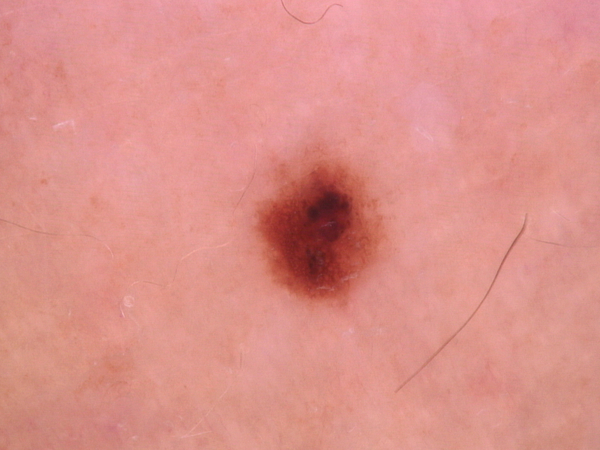
\includegraphics[scale=0.4]{ISIC_0024335.jpg}\newline
    \end{figure}
    \item \textbf{Melanoma:} A serious skin cancer that develops in the cells producing melanin. In the model, it is diagnosed as class 1 (Figure 2).
    \begin{figure}[h]
    \caption{Melanoma Image}
    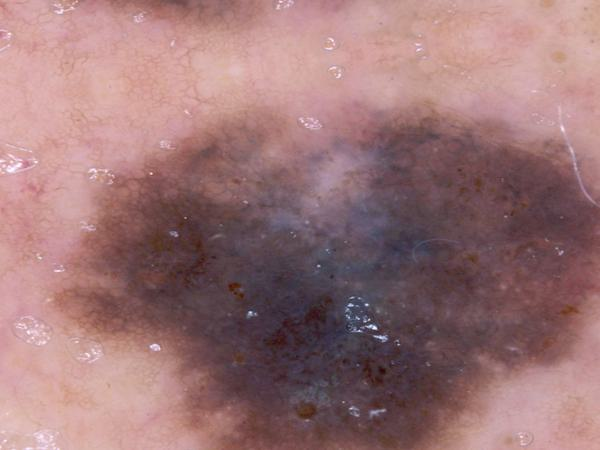
\includegraphics[scale=0.4]{aug_mel__10_3539.jpg}\newline
    \end{figure}
 
\end{enumerate}

The algorithm of the model and its technique to analyze images and classify them is heavily inspired by a dermoscopic method called “ Pattern Analysis”.
\newline
Pattern Analysis is the method preferred by many expert dermoscopists to diagnose pigmented skin lesions in order to differentiate benign melanocytic nevi from melanomas. The method requires assessing many lesion patterns simultaneously. To access melanocytic lesions, two different visual characteristics are seen within a lesion: Global pattern and local features. For benign melanocytic lesions, they typically have reticular, globular, homogeneous, or parallel furrow patterns. They may have a complex pattern, but it is usually regularly distributed symmetrically. Local features include pigmented network evenly spaced fading out, dots and streaks distributed regularly, or symmetrical blotches \cite{DermNet}.
\newline
Melanomas usually have multicomponent patterns (3 or more), unspecific, structureless, and irregular patterns that are not evenly distributed. Local features include atypical pigment network, dots/globules distributed irregularly, asymmetrical blotches, five or six colors (black, brown, tan, gray, blue, red, white), blue-white veil, and irregular lines, dotted vessels, or parallel ridge patterns \cite{DermNet}. 
\newline
In general, benign lesions have few colors, a regular structure and are symmetrical in pattern. Malignant tumors often have several colors, disordered structure and asymmetric pattern.

\subsection{Machine Learning}
In the proposed model, feature extraction techniques were integrated with CNN using dermoscopic images to detect melanoma. Hu moments and color histograms are feature extraction techniques in image processing. Hu Moments are geometric descriptors used to characterize the shape of an object in an image. It is also the weighted average of image pixel intensities. These moments capture the area, centroid, and orientation of an object. Color histograms represent the distribution of colors in an image. They quantify the frequency of the appearance of certain colors. Generally, feature extractions can help capture the overall shape and color profile; thus, it analyzes global patterns. The global feature descriptors are used to combine with a neural network in order to analyze the image as a whole (both local and global) \cite{pham2021ai}
\newline
\newline
A neural network will be designed in order to classify the two pigmented skin lesions. Neural networks or artificial neural networks (ANNs) is a fundamental subset of machine learning and is the core of deep learning algorithms. Mimicking the function of a human neuron, a deep learning neural network has an input layer, which receives data like the dendrite, a hidden layer where computation and weight adjustment occur like the cell body, and the output layer which transmits the final processed information like the axon of a nerve cell. These different layers work together to recognize, classify and describe the objects within the data \cite{IBM}.
\newline
\newline
The proposed model is a supervised learning as it presents the dataset of pigmented skin lesions with their labels to be trained by the classification algorithm. The data will be separated into different categorical classes and predictions will be made according to the inputs and labels.
\newline
\newline
Convolutional Neural Network (CNN) is a deep learning algorithm suited for data processing image recognition. A CNN model consists of multiple layers including the convolutional, pooling, and fully connected layers to effectively process the data and its visual components \cite{Mishra_2020}. 
\newline
\newline
The convolution layer is generally responsible for detecting patterns in the input data, such as edges, colors, or textures. This layer has a filter matrix where it slides over the image and computes the dot product to detect patterns. The filter is derived to look for patterns and to produce a feature map (convolved feature) to transform the input data and make it easier for the network to understand what to do. An example is Conv2D layers, or a two-dimensional convolutional layer, used for processing two-dimensional images. Convolutional Layers in CNN can add detailed textural and pattern information for local feature analysis. The filter in the layer passes over the image and performs localized convolution operation, which multiplies the filter’s values by the original pixel values in a small region of the image. CNN often uses layer hierarchies which learn basic features like edges at first, but get deeper into more complex patterns \cite{Mishra_2020}. 
\newline
\newline
The pooling layer serves to reduce the spatial dimensions (height and width) of the incoming feature maps from the previous layers, such as a convolutional layer. It performs a down-sampling operation to achieve this reduction. The input is a rectified feature map typically produced from the preceding activation function applied within a convolution layer. It goes through a down-sampling operation that reduces the dimensionality of the feature map. In each part of the map, it looks for the maximum value to find the most valuable or important part of the section. It then uses different filters to identify parts of the images like edge, corner, body, etc. MaxPool2D layers are used to process the 2d images from the dataset \cite{Mishra_2020}. 
\newline
\newline
The fully connected layer interprets the features extracted by previous layers to make a final prediction or classification. Before reaching the fully connected layer, the output from the last pooling or convolutional layer is transformed. This process, known as flattening, converts the 2D feature maps into a 1D vector. If the feature maps are multidimensional, they are all unrolled or reshaped into a single long vector. The flattened matrix from the pooling layer is fed as the input to the fully connected layer to classify the image. Dense layers are activated where the flattened vector is then fed as input to the fully connected layer. This layer consists of neurons that have learnable weights and biases. Each neuron in a fully connected layer receives input from all the elements of the flattened vector. In the context of binary classification, the fully connected layer will use sigmoid (for binary classification) to output probabilities within the 2 classes \cite{Mishra_2020}.
\newline
\newline
Activation functions calculate the output of the node based on its inputs and weights. The function's output decides how much signal from the neuron will be passed forward to the next layer in the network. A common example includes the ReLU (Rectified Linear Unit) function. The ReLU layer processes small amounts of data in each image with activation function. Negative pixels are set to 0. This step also introduces non-linearity to the network. Output is a rectified feature map looking at just the important features of an image. In detail, it scans images for locating features where black denotes negative and white denotes positive values \cite{GeeksforGeeks_2019}. ReLU is also chosen as it helps with the vanishing gradient problem: when the gradients of the activation function become too small during backpropagation, leading to slow or stalled learning in deep neural networks.why use bigger fonts?
\newline
\newline
Back Propagation happens during the training phase, when CNN uses a loss function to calculate the error in its prediction compared to the actual result. The network then applies the backpropagation algorithm: it propagates the error backward through the network, adjusting the weights of the filters and neurons via gradient descent. This happens over again in a loop until its last epoch or when early stopping is activated \cite{Roy_2020}.
\newline
\newline
Gradient Descent is an optimization algorithm in back propagation used to minimize the loss function by iteratively moving towards the minimum value of that function. It measures the difference between the model's predictions and the actual data. During training, gradient descent adjusts the model's parameters (like weights) to find the point where the loss function outputs its lowest value, which corresponds to the model's best performance \cite{Roy_2020}. 
\newline
The learning rate is a crucial hyperparameter in this process; it determines the size of the steps taken towards the minimum. A smaller learning rate means taking smaller steps, which can lead to a more precise convergence but may increase the time taken to find the minimum. Conversely, a larger learning rate speeds up the process but risks overshooting the minimum.
\newline
Hyperparameter tuning is a critical process in machine learning that happens after initial results and attempts to analyze how a model behaves. It finds the most effective combination of hyperparameters for a given model. Hyperparameters are the external variables of a model that are not learned from data but are set prior to determine the network structure and to optimize the model’s performance \cite{Amazon_1978}. 
\newline
\newline
After the model is trained, the proposed work will compare their model’s performance with studies and pre-trained models to see whether it can outperform. Pre-trained models are deep learning models that have already been trained on large datasets to accomplish specific tasks such as feature extraction, classification to derive insights from large amounts of data. Essentially, implementing a pre-trained model is using someone else’s work as the structure of the model, the layers, etc have already been designed. This is also known as transfer learning, where a model trained on one task is used as the starting point for a model on another task. 

\section{Prior and Related Work}

\subsection{Global Features}
Global Feature descriptors are used to quantify the image as a whole making sure it gets a general analyzation without the concept of only paying attention to the interest points; in contrast with CNN models which only look for local features.
\newline
\newline
Shetty et al. demonstrated the use of global features like Hu Moments, Color Histograms, and Haralick textures for skin lesion analysis \cite{shetty2022skin}. Ramesh et al. also utilized similar global features for plant disease detection \cite{ramesh2018plant}. My proposed model incorporated global features like color histograms and Hu moments to enhance the understanding of skin lesions, following the precedent set by Shetty et al. and Ramesh et al. This contributes to the argument that incorporating global features alongside image data enhances analysis by combining a general structure with points of interest.
\newline
\newline
Global features are computationally efficient and provide better interpretability than Srinivasu’s model that focused on MobileNetV2 and LSTM because they are designed to analyze sequential data and focus on local patterns, whereas global features provide a more holistic understanding of the skin lesions, capturing both local and overall characteristics \cite{srinivasu2021classification}.
\newline\newline
Other techniques in feature detection that are not used in the proposed study include Kernel Space and fuzzy modeling. The proposed study intentionally avoided using complex techniques like Kernel Space and fuzzy modeling to maintain a straightforward and interpretable model, as well as to focus on specific feature extraction and classification approaches without introducing unnecessary complexity.

\subsection{Image Segmentation}
Image segmentation is the process of dividing an image into meaningful and visually distinct regions or objects for further analysis. Its exploration of image segmentation and ensemble methods was explored by Codella, including the combination of ResNet50 and VGG16, highlighting the diversity of approaches in the field \cite{codella2018skin}. \newline
Codella performed lesion segmentation by mask images resulting. The masks are binary images where it separates the part of the image that is the actual skin lesion and the part that is the background. While these methods offer nuanced insights, my proposed model did not use image segmentation; its focus was on understanding the fundamental aspects of machine learning model construction, thus opting for a more streamlined approach.

\subsection{Data Augmentation}
Data augmentation has emerged as a pivotal technique in addressing overfitting and class imbalance, as noted by Shahin et al. and Srinivasu et al \cite{shahin2018deep} \cite{srinivasu2021classification}. By artificially enlarging the training set with variations of input images (without new data collection), data augmentation not only enhances model robustness but also ensures a more balanced representation of different lesion types. Augmentations included, but were not limited to, rotations and transformations. \newline \newline
Shetty et al.'s findings corroborate this, indicating that models equipped with data augmentation capabilities tend to learn more distinguishing features, thereby improving accuracy.My proposed model's incorporation of data augmentation aligns with these findings, aiming to improve accuracy while overcoming the limitations posed by a finite number of images \cite{shetty2022skin}. \newline \newline
Data augmentation is used in the proposed model. Resampling was also used with data augmentation techniques such as ImageDataGenerator. They both help increase the variability in the dataset. Augmentation includes shift, zoom, and rotate.

\subsection{BatchNormalization, Custom Loss function}
The implementation of BatchNormalization and a custom loss function, as investigated by Pham et al., represents another facet of model optimization. Such optimizations are crucial in fine-tuning the model performance and ensuring consistency in results. Batch normalization is used to stabilize the training process of the model. Specifically it helps solve vanishing gradients; where gradients in backpropagation become extremely small, hindering weight updates and slowing down training. BatchNormalization normalizes activations to reduce the range of values for more consistent gradient flow. Pham et al introduced their own custom loss function (CLF) by separately calculating the loss of mean squared error on positive and negative class images and essentially tallying them up. The CLF was not implemented in the proposed model due to the complexity of the architectural structure \cite{pham2021ai}. 

\subsection{Pre-trained models and transfer learning}
Hosny et al. used pre-trained AlexNet with transfer learning, illustrating the effectiveness of combining global feature descriptors with deep learning techniques in skin lesion classification \cite{shetty2022skin}. Shetty et al. also technically implemented pre-trained models by comparing with other investigators’ models in order to prove that their model was superior. In my case, I used pre-trained models (ResNet50 and VGG16) because I am able to thoroughly compare the performances between my proposed CNN + feature extraction model and other people’s models on the same dataset to see which one obtained the best results.

\subsection{Apps}
In practical applications, tools like FotoFinder and the DermEngine platforms demonstrate the real-world implementation of these technologies. Both platforms provide total body photography to scan and analyze skin lesions. Fotofinder Vexia has an AI assisted video dermoscopy function while the ATBM master combines total body photography and video dermoscopy . While not compatible through mobile apps, FotoFinder does display visual characteristics of skin lesions \cite{humans.txt}.\newline \newline
DermEngine is an AI dermoscopic software compatible on iOS, android, TV, web, etc. It uses teledermatology to help patients submit images, taken by an attachable camera on the phone, through the patient app or connect directly via video consultation. Images are kept securely as they are reviewed by medical experts. However, the app does not independently detect and diagnose skin lesions\cite{Inc.}
\newline \newline
There are also many online apps people can purchase or subscribe to diagnose skin lesions with their cellular phones such as Dermoscopy Self Assessment and Mole Checker Skin Dermatology.


\section{Methods}
\begin{enumerate}
    \item \textbf{Image Preprocessing:} The dataset used, HAM10000 (Humans Against Machines), is an academic training set consisting of 10015 dermatoscopic images. It was created to address challenges in training neural networks for automated diagnosis of skin lesions, particularly issues related to the small size and lack of diversity in existing dermatoscopic image datasets. \newline \newline
    Unfortunately, like many datasets in the medical field, the HAM10000 dataset is imbalanced in the number of images per class. For instance, out of 10015 images, 6705 of them are from ‘nv’, while only 1113 images are diagnosed with melanoma \cite{tschandl2018ham10000}. Oversampling, a type of resampling, was used to duplicate the melanoma images since it was the minority class \cite{KDnuggets}. In this model, images were resampled in two different formats. \newline

    The first strategy involved the horizontal and/or vertical flipping of each image. Essentially it’s a subtle and effective way to introduce mirror images. This approach is particularly beneficial in medical imaging, where the orientation of an image often does not alter the essential characteristics of a lesion. The key reason for limiting this resampling to three iterations was to avoid redundancy. Excessive flipping could lead to duplicate images, which might cause the model to memorize specific instances rather than learning to generalize from broader patterns. Thus, flipping was used judiciously to enhance the dataset's diversity without compromising its quality, ensuring that the model remains robust and reliable in identifying lesions from various orientations. \newline \newline
    The second method is where ImageDataGenerator is used to increase the number of samples and to increase the dataset variability. ImageDataGenerator, a key tool in our approach, applies geometric transformations such as rotation, shift, zoom, and flip during duplication, carefully chosen to mimic the diverse appearances of skin lesions \cite{TensorFlow}. This method was selected for its ability to introduce a wider array of realistic variations that skin lesions might exhibit in real-world settings. Each of these transformations was carefully chosen to mimic the diverse ways in which skin lesions can appear, thereby preparing the model to handle real-life diagnostic scenarios effectively. Rescaling and zooming cater to variations in lesion size, rotation and translation address different lesion orientations, and the 'reflect' fill mode ensures the model is exposed to various edge and boundary conditions. This overall helps prevent overfitting and improve model robustness. It also improves performance on minority classes to ensure a more balanced error rate. In short, existing samples were duplicated with minor alterations to balance the dataset between the classes, part of it being data augmentation itself. \newline \newline
    Other oversampling techniques include color space transformations, kernel filters, random erasing, and mixing images. However, only geometric transformations were applied because other transformations can hinder the performance of the model as it might generate unrealistic and inaccurate photos where important details can be left out. In summary, I employed a combination of resampling and data augmentation techniques. While data augmentation enhances dataset variability without new data collection, resampling, particularly oversampling, helps balance the dataset by duplicating minority class images like ‘mel’ to match the number in ‘nv’. This approach ensures a balanced dataset without introducing exact duplicates.
    \newline
    \item \textbf{Data Shuffling and Splitting:} After the data has been augmented and combined, it is shuffled to make sure there is no risk of a particular set having an overwhelming majority of images in a specific class over one another. Tran\_test\_split is imported from scikit-learn in order to split the entire dataset into 3 categories: Train, Validate, and Test \cite{scikit}. \newline The training dataset is the sample of data used for the model to see and learn from it. \newline The validation set helps evaluate a given model every epoch after it finishes with the training batch set; It is used to fine-tune hyperparameters. The model doesn’t learn from it. Essentially, it is practice for the test set because it is a good indicator on whether the model has actually learned something useful from the training data. Otherwise it is overfitting. \newline The test set is only used once after the model is fully trained where it evaluates the completed model, such as the accuracy, precision, recall, etc \cite{Shah_2020}. The ratio of images in each category was set to 60, 20, 20\%. The train needs to have a much higher quantity of data compared to the validate test because the model needs to substantially recognize patterns and establish a boundary where it can easily tell the difference between classes. 
    \newline
    \item \textbf{Feature Extraction:} Global feature descriptors were used to quantify the image as a whole making sure it gets a general analyzation. This step is connected with the global pattern detection algorithm in pattern analysis used by Dermatologists. The color of the skin lesion image is quantified using a Colour Histogram. The shape of the skin lesion is quantified using Hu Moments. These features are chosen because the color and shape are one of the main properties that dominate in the lesion zone \cite{pham2021ai}. \newline \newline
    The feature extraction works with one image at a time, extracting the shape and color, then concatenating them into a single global feature. Both extraction techniques were combined and integrated into CustomDataGenerator that activates when the training, validating, and testing set is initialized. For every image in the set, they will be processed including their global features which are then taken into the feature input pathway where global features are processed in the CNN model. The pathway compromises dense layers from the fully connected layer to interpret the concatenated global features. Fully connected layers are responsible for processing non-spatial numerical features and identifying complex patterns and relationships to process global features.
    \newline
    \item \textbf{CustomDataGenerator:} In managing extensive image datasets within machine learning frameworks, particularly when integrated with TensorFlow and Keras, the development of the Python class CustomDataGenerator offers a significant advancement over traditional methods such as the `load\_data` function that was initially planned in the proposed model. Unlike `load\_data`, which typically loads entire datasets into memory, leading to inefficiency and potential system strain, CustomDataGenerator employs a more sophisticated batch processing approach. This method optimizes memory usage by loading data in subsets as required, a crucial feature for handling large datasets and enabling real-time data augmentation. \newline \newline The choice to develop CustomDataGenerator was driven by the limitations observed in the `load\_data` function. While `load\_data` provides basic preprocessing capabilities, it lacks the flexibility to accommodate complex, custom preprocessing steps that are often essential for specific datasets. CustomDataGenerator addresses this gap by allowing the integration of advanced preprocessing operations such as specialized normalization and resizing, directly within the data pipeline. Additionally, the flexibility to integrate with various image processing libraries opens avenues for more sophisticated image analysis techniques, further enhancing data quality for model training. \newline \newline Furthermore, this approach reflects recent academic insights into machine learning data processing, underscoring the importance of custom solutions for data handling in specific applications, particularly in specialized fields like medical image analysis. The data augmentation capabilities offered in CustomDataGenerator conserve memory and enhance the dataset. On-the-fly augmentation from CustomDataGenerator was only implemented in the training dataset to prevent data leakage and ensure realistic evaluation by evaluating the model’s generalization ability on more real data. By enabling more tailored data preparation and management, CustomDataGenerator not only ensures efficient memory usage but also potentially improves model training effectiveness by providing more accurately preprocessed data. (See Appendix for more details)
    \newline
    \item \textbf {Building the Model:} The proposed work designed a CNN model to train, validate, and test the image dataset. To build the CNN, Tensorflow and Keras libraries were used to build and implement the model. \newline
    In medical image classification, Convolutional Neural Networks (CNNs) excel in image classification due to their architecture and functionality. They contain additional layers before the fully connected layer where spatial hierarchies are learned. Other methods that could be used include Random Forests, and Support Vector Machines. However, RFs and SVMs are not inherently suited for high-dimensional data like images and require manual feature engineering. Unlike CNN, they don’t scale well to large datasets \cite{Khoong_2021}. The designed hybrid model comprises two distinct components, each targeting a different aspect of image analysis. \newline
    The first segment, the image pathway, processes raw image inputs through convolutional layers that detect local features, coupled with pooling layers that aim to reduce dimensionality. This configuration is specifically devised to extract and prioritize critical image data attributes. The network integrates four convolution layers and two pooling layers, arranged in segments with two Conv2D layers followed by a MaxPool2D layer. Hierarchical feature learning is achieved through the dual Conv2D layers, enhancing feature complexity and diversity, while the Pooling Layers contribute to dimensionality reduction, thus curtailing computational demands and mitigating overfitting risks. \newline
    The second segment focuses on global feature processing. Dense layers adept at handling non-spatial data interprets and amalgamate high-level data abstractions, independent of specific spatial image locations. Initialization of the 'feature\_input' utilizes Keras' Input layer, defining the input shape corresponding to the global feature vector length, extracted using image moments and color histograms. A sequence of three dense layers with descending neuron counts then processes these global features, each proceeding layer augmented with BatchNormalization to stabilize learning by adjusting and scaling activations.\newline
    This dual-pathway approach, synthesizing local and global features, furnishes the model with a comprehensive image understanding. Local features excel in capturing intricate details like edges and textures, while global features impart contextual and overarching image characteristics. Such integration fosters enhanced model accuracy and robustness, particularly in image classification and object detection tasks.\newline 
    Upon finalizing the model design, both pathways converge, concatenating the flattened output from the local features with the global features processed by dense layers to create a unified feature vector. The concatenated vector is then brought to one last dense layer where sigmoid activation is used to distribute a probability value between 0 (negative class) and 1 (positive class).
    \newline
    \item \textbf {Hyperparameter Tuning:} Hyperparameter tuning was implemented where values were adjusted or established for better model evaluations and results. It is also to prevent overfitting - when a model memorizes the noise and fits too well in the training set, it significantly underperforms in the validate, test set, or unseen data. This was a big obstacle in designing the hybrid model due to insufficient training data or imbalance training data before I resampled. The batch\_size was strategically set to 32, optimizing memory usage and ensuring efficient training by processing subsets of the training data sequentially. This choice balances computational resource usage with the need for model accuracy and generalization. \newline The confidence threshold is a key hyperparameter, as it is adjusted to 70\% meaning the minimum score that the model will consider the prediction to be a true prediction is 70\% for melanoma detection. This was changed to reduce false positives, and to adjust to a medical field setting as decisions must be substantially confident before finalizing. It was also to balance between sensitivity and specificity. Adjusting the threshold in medical diagnostic tests is a critical decision that balances the risks of false negatives (type II error) and false positives (type I error), each carrying its own set of consequences. In scenarios where missing a diagnosis (false negatives) could lead to severe health deterioration, such as in cancer detection, a lower threshold may be preferred to ensure high sensitivity. This approach captures more true positive cases but at the risk of increased false positives. Conversely, in situations where the consequences of over-treatment are significant, such as unnecessary surgeries or treatments, a higher threshold might be set to enhance specificity, thereby reducing false positives but potentially increasing false negatives. \newline
    Keras Tuners, a submodule of Keras, facilitated efficient hyperparameter tuning. This approach contrasts with the less effective trial-and-error method, optimizing key hyperparameters such as filters in Conv2D layers, units in dense layers, dropout rate, and learning rate. The learning rate was meticulously reduced as the model showed improved performance at lower rates. Additionally, the training was limited to 10 epochs to prevent overfitting, ensuring that the model generalizes well to new data without memorizing the training set. \newline 
    Regularizers L1 and L2 were both experimented and unsuccessful as they over-regularized the model. The accuracy was heavily reduced and increased loss. In short, the model didn’t perform as well. The purpose of regularizers is to penalize large weights in the model to prevent overfitting. Within the hybrid model, using these regularizers might have led to over-regularization, where the model becomes too simple to capture the complexity of the data, reflected in lower accuracy and higher loss. The introduction of these regularizers appeared to excessively penalize the model’s weights, leading to underfitting. \newline
    Tanh function was also experimented to replace ReLU. The tanh function outputs between -1 and 1; it is a scaled version of sigmoid. However, it led to an increased loss and lowered accuracy. A reason being ReLU is known for being less computationally expensive and solving the vanishing gradient problem by not saturating as drastically, and with constant and bigger gradients than Tanh. Replacing it eliminated the problem, where gradients become too small for effective learning in deep networks \cite{Gupta_2021}.\newline 
    Adam was set as an optimizer; ReLU and sigmoid were used as activation functions. Adam helps adjust the learning rate throughout the training process for each parameter individually. Sigmoid outputs a probability value of the input belonging to one of two classes between 0 and 1. It is ideal for binary classification as it’s better mapped for two classes: closer to 0 meaning negative; closer to 1 meaning positive diagnosis. Softmax is a more complex procedure where it converts the output for each class into probabilities that sum up to 1 \cite{Basta_2020}. 
    \newline
    \item \textbf {Transfer Learning:} Pretrained models such as VGG16 and ResNet50 were added to compare their performance with the designed hybrid model. The work plans to compare ResNet50 with the dermoscopic CNN, as well as with studies that have used binary CNN for melanoma and nevus detection. \newline 
    ResNet50 and VGG16 are two prominent architectures in the field of Convolutional Neural Networks (CNNs), widely used in deep learning for image classification and recognition tasks. ResNet50 is part of the Residual Network (ResNet) family developed by Microsoft. It contains 50 layers, including convolutional, shortcut connection, and fully connected layers. VGG16 was developed by Visual Graphics Group from Oxford, hence the name VGG. It contains fewer layers at 16 that have weights; this includes 13 convolutional layers and 3 fully connected layers. It uses 3x3 convolutional filters with a stride of 1, and max pooling is used throughout. ResNet50 is deeper than VGG16, but due to its efficient use of parameters and skip connections, it is less prone to overfitting and more scalable. VGG16 has a larger number of parameters, making it more memory-intensive, whereas ResNet50, despite its depth, is more efficient. \newline
    Both models represent distinct approaches in the field of deep learning and are widely adopted in transfer learning due to their proven effectiveness and differing strengths. By comparing these established models with the work’s hybrid model, insights into the relative performance, efficiency, and scalability of the hybrid model can be observed. This comparison is particularly valuable for assessing the hybrid model's effectiveness in handling the specific challenges of the image dataset used in this project, including its ability to generalize and perform under varying data conditions. \newline
    In addition to two pre-trained models, a CNN standalone model was used to compare its metrics. The CNN model was the initial draft of the project before feature extractions were added and concatenated with the local features from the convolution and pooling layers. The purpose is to show how much of an improvement manual methods of feature extraction are for better results. Some hyperparameters like learning rate, convolutional kernel, and pool matrix size were kept for consistency. However, the neurons were changed as it was suggested from Keras.tuners. 

\end{enumerate}

\section{Evaluation Metrics}

The model is evaluated with several metrics in order to provide a comprehensive view of the model’s performance: precision as the ratio of correctly predicted positives to the total positive predictions, recall/sensitivity as the ratio of correctly predicted positives to the actual positive observations, F-1 score which computes the harmonic mean of precision and recall, accuracy marks the number of correct predictions, and specificity which measures the proportion of true negatives. These metrics align with the goal of designing an accurate model (Figure 3 displays the metric formulas).

\begin{figure}[h]
\centering
\caption{Accuracy, Precision, Recall, F-1, Specificity}
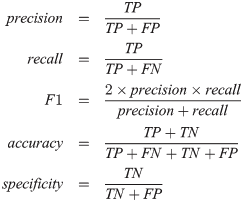
\includegraphics[scale=0.5]{Formulas.png}\newline
\end{figure}

Confusion Matrix will be used to give a holistic view on its true and false predictions (Figure 4).

\begin{figure}[h]
\centering
\caption{Confusion Matrix}
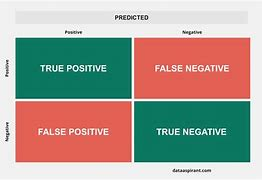
\includegraphics[scale=0.5]{ConfusionMatrix.jpg}\newline
\end{figure}

Shahin et al. similarly recorded those metrics, but they performed multi-class; therefore, collecting the average precision and recall for each class \cite{shahin2018deep}.
Training and Validating accuracy graphs and loss graphs will be plotted. In addition, the ROC curve will be implemented. These metrics were also recorded in the Shetty et al. and the Pham et al. study \cite{pham2021ai}.
The ROC curve is a graph that plots to visualize the evaluation of the true positive rate (Recall) against the false positive rate at different threshold settings. Basically, it plots different confusion matrices at different thresholds. Sometimes a diagonal dotted line is sketched, but that represents when the true positive and false positive rate are equal (0.5 AUC). Optimally, the curve should occupy the top and left side of the graph. It should be well above the diagonal line because it represents a higher true positive than false positive rate at various thresholds. ROC curves can help visualize how many false positives are willing to be sacrificed to increase true positivity. On the bottom left of the graph is when the threshold is 1.0 (100\% probability required for true diagnosis). Everything is diagnosed as negative because it is almost mathematically impossible for a model to have a 100\% probability of classification. On the top right of the graph is when the threshold is 0.0. This means everything is diagnosed as positive; it also means there is an equal true positive and false positive rate. The Area-under-the-curve (AUC) is the probability that a randomly chosen positive instance is ranked higher than a randomly chosen negative instance. An AUC of 1.0 suggests the model will always be able to distinguish between a randomly chosen positive and negative instance. This is an important metric because it helps analyze whether the model understands the difference between a benign mole and a melanoma. \newline \newline
The loss graph shows the error between predicted and actual outputs during training and validating. The y axis is the loss value; the x axis is the number of epochs. A decreasing loss over epochs suggests that the model is learning and converging towards a set of parameters that minimize the error. If the training loss continues to decrease while the validation loss begins to increase, it is a sign of overfitting. The model would then be learning to memorize the training data, losing its ability to generalize to unseen data. Both graphs remaining high represent underfitting. \newline
The accuracy graph shows the proportion of correct predictions over all instances. It helps visualize how effectively a model is learning over epochs. If the training accuracy is significantly higher than the validation accuracy, it is a sign of overfitting because the model is learning to memorize instead of adapting. 
\newline
Both the loss and accuracy graph helped interpret an appropriate value for early stopping and learning rate. Early stopping can help prevent overfitting; the learning rate can help adjust at the pace where minimum loss is achieved. 

An alternative method included Matthew’s correlation coefficient - a statistical measure to provide a balanced evaluation of binary classification performances; useful in case of imbalanced datasets. However, resampling was already used to balance the dataset among the two classes of pigmented skin lesions.

\section{Results and Discussion}
\subsection{Results}
In this study, four different machine learning models were evaluated using a variety of metrics to assess their performance in skin lesion classification. The key metrics included Accuracy, Precision, Recall/Sensitivity, Specificity, F-1 Score, and Area Under the Curve (AUC). These metrics were chosen for their relevance in the field of medical diagnostics, where accuracy and reliability are paramount. Table 1 displays the evaluation metrics data among the four models
\subsubsection{Evaluation Metrics Data}
\begin{table}[h]
\centering
\caption{Evaluation Metrics Data}
\scriptsize
\setlength\tabcolsep{3pt} 
\begin{tabular}{|l|c|c|c|c|}
\hline
\textbf{Metric} & \textbf{CNN} & \textbf{CNN+Feat. Ext.} & \textbf{ResNet50} & \textbf{VGG16} \\ \hline
Test Acc. & 81.39\% & 86.50\% & 74.87\% & 82.33\% \\ \hline
Prec. & 0.86 & 0.85 & 0.85 & 0.92 \\ \hline
Recall/Sens. & 0.65 & 0.88 & 0.5 & 0.6 \\ \hline
Spec. & 0.90 & 0.84 & 0.91 & 0.95 \\ \hline
F-1 & 0.74 & 0.87 & 0.63 & 0.73 \\ \hline
AUC & 0.895 & 0.931 & 0.840 & 0.921 \\ \hline
\end{tabular}
\end{table}


\subsubsection{Confusion Matrices}
\begin{table}[h]
\centering
\caption{Confusion Matrices}
\scriptsize
\setlength\tabcolsep{3pt} 
\begin{tabular}{|l|c|c|c|c|}
\hline
\textbf{Metric} & \textbf{CNN Model} & \textbf{CNN + Feature Extractions} & \textbf{ResNet50} & \textbf{VGG16} \\ \hline
True Positive & 868 & 1182 & 880 & 802 \\ \hline
False Negative & 473 & 159 & 671 & 539 \\ \hline
False Positive & 137 & 209 & 122 & 66 \\ \hline
True Negative & 1204 & 1172 & 1219 & 1275 \\ \hline
\end{tabular}
\end{table}

\begin{figure}[h]
\caption{Comparative Performance of Machine Learning Models on Dermoscopic Image Analysis}
\centering
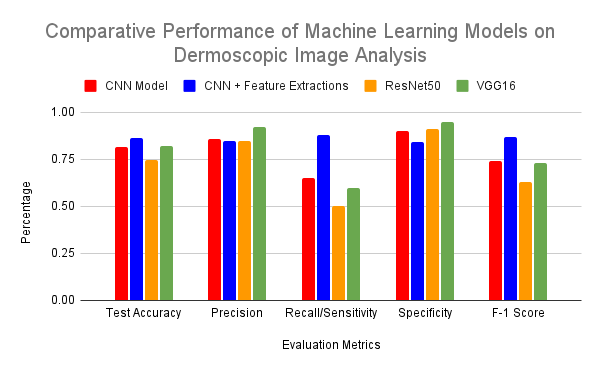
\includegraphics[scale=0.4]{Comparative Performance of Machine Learning Models on Dermoscopic Image Analysis.png}\newline
\end{figure}

The inclusion of a graph chart (Figure 5) in the results section provides a visual representation of the performance metrics across the models. It allows for a quicker and more intuitive comparison of model performances, making it easier to identify trends and differences. In the graph above, it effectively highlights the trade-offs between accuracy, precision, recall, specificity, and f1 score. Metrics were chosen to showcase the overall balance of a model's performance. \newline
The CNN + feature extractions model excels with the highest accuracy at 86.50\%, showcasing its exceptional proficiency in accurately classifying skin lesions. The VGG16 is a close second with an accuracy of 82.33\%, trailed slightly by the CNN standalone model with an accuracy of 81.39\%. ResNet50, however, had the lowest accuracy of 74.87\%.
In terms of precision, the standalone CNN model leads at 0.86, indicative of its reliable positive predictions. The precision for CNN + feature extractions and ResNet50 is marginally lower at 0.85 each, while VGG16 demonstrates the highest precision at 0.92. Regarding recall, VGG16 stands out with a notable rate of 0.60, efficiently identifying true positive cases. CNN + feature extractions follows with a recall of 0.88, whereas the CNN Model and ResNet50 exhibit lower recalls of 0.65 and 0.50, respectively. The VGG16 showcased the highest specificity at 0.95, most adept at identifying true negatives. Resnet50 and CNN standalone displayed strong specificity as well at 0.91 and 0.9 respectively. CNN + feature extractions surprisingly scored the lowest at 0.84. \newline

For the F-1 score, CNN + feature extractions had the highest at 0.87 which indicates a well balanced performance between precision and recall. The other 3 models had noticeably lower f-1 scores. While their specificities were all higher than the CNN + feature extraction, their sensitivities were much lower. The CNN itself scored 0.74; and followed by VGG16 at 0.73. ResNet50 had the lowest F-1 score at a measly 0.63. \newline
Within the test set, there were 2682 images in total; exactly half of them were labeled positive and negative. The VGG16 model detected the most true negatives at 1275, but the second highest false negatives at 539. Moreover, it had the lowest true positives at 802; but fortunately had the fewest false positives at 66. \newline ResNet50’s performance showed the second highest true positives at 880, second highest true negatives at 1219, and the second lowest false positives at 122. However, it had the highest false negatives at 671 images accounting at 25\% of the test set. \newline The CNN standalone model had the third highest true positives at 868, 2nd lowest false negatives at 473, second highest false positives at 137, and the second lowest true negatives at 1204. The CNN model showed a decent balance between the two classes; however, the CNN + feature extraction Model by far had the overall best balance of metrics. It may have had the lowest true negatives (1172) and highest false positives, but it had the most true positives at 1182 and the lowest false negatives at 159.
\newline
\subsubsection{Graphs}
\begin{figure}[h]
\caption{ROC Curve}
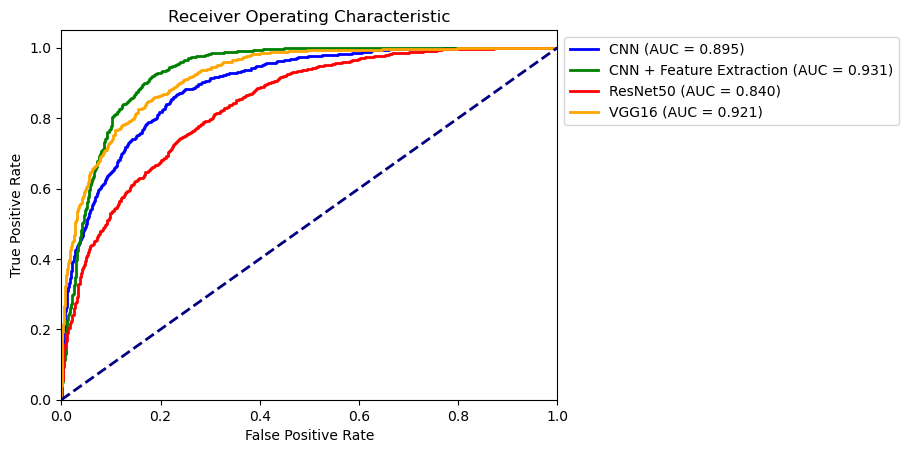
\includegraphics[scale=0.4]{ROC.png}\newline
\end{figure}
The Receiver Operating Characteristic (ROC) curve (Figure 6) illustrates that the CNN + feature extraction model, with an AUC of 0.931, demonstrates a high probability — 93.1\% — of accurately distinguishing between positive and negative cases at various decision thresholds, thanks to its integrated additional features. This model, alongside VGG16 which showcases a similar AUC of 0.921, indicates their comparable effectiveness in classification performance throughout the range of thresholds. \newline
The standalone CNN model, with an AUC of 0.895, shows robust performance on its own. The marginal gain in AUC when additional features are integrated suggests that the fundamental CNN framework is adept at discerning critical details, and the enhancement from extra features, while beneficial, builds on an already solid foundation. \newline
ResNet50's AUC of 0.840, while modest in comparison, still demonstrates competent classification capabilities. This outcome points to potential enhancements that could be made, possibly through model optimization, dataset expansion, or improved data preprocessing techniques.

\begin{figure}[h]
\caption{Training and Validating Accuracy for Multiple Models}
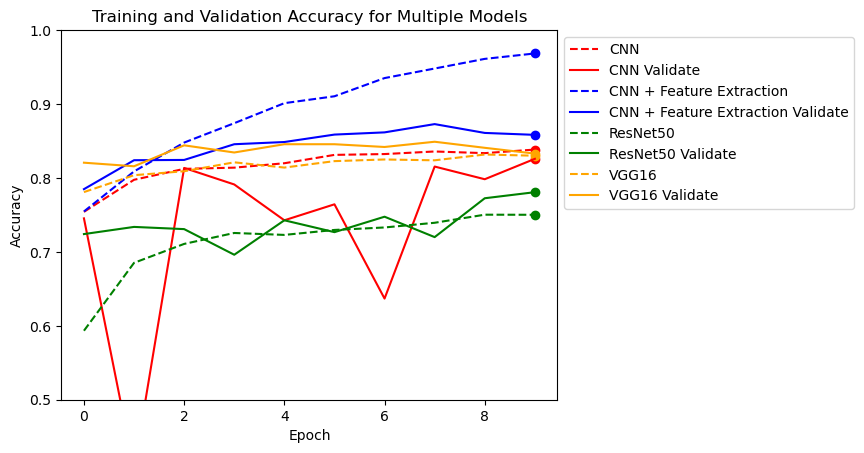
\includegraphics[scale=0.4]{AccuracyEpochs.png}\newline
\end{figure}

The observed results in the training and validation accuracy across the four models can be attributed to their specific architectures and learning capacities (Figure 7). 
ResNet50's at lowest accuracy overall as it never passed 80\%, but both train and validate sessions are observed to be increasing slowly over 10 epochs; it hints at a complex model architecture that may require more data or refined tuning specific to the task at hand to leverage its full potential. ResNet50, known for its depth and capability to learn complex patterns, might not have been fully utilized due to insufficient data or the need for more fine-tuning for the specific task. This underutilization could lead to its suboptimal performance. \newline
On the other hand, the CNN model training session had a higher accuracy and slowly increased over epochs but showing a significant drop and erratic fluctuation in validation accuracy points towards overfitting. This discrepancy reveals the model's tendency to memorize the training dataset intricacies rather than learning generalizable patterns, a classic overfitting scenario in machine learning. \newline
The VGG16 model exhibited a steady ascent in the training accuracy. However, surprisingly its validating accuracy was slightly above. Both of them hovered around 80\%. However, both graphs, but more noticeably the validation accuracy graph, is a bit more fluctuating. Even though it generally increased it sometimes decreased along the way between epochs. \newline
Both the VGG16 and CNN + feature extraction models exhibit a steady ascent in training accuracy, crossing the 90\% threshold, which signals effective learning processes. Nonetheless, a slight dip in validation accuracy towards the later training epochs may signal the commencement of overfitting, as the models potentially begin to fit too closely to the training data's nuances, which do not extrapolate to unseen data. \newline
The CNN + feature extraction models demonstrated the highest performance. The training accuracy increased at the most stable and highest rate as it surpassed 90\%; its max value reached 96.84\%. The validating accuracy, still the highest (slightly hovering VGG16), did perform noticeably worse as it never surpassed 90\%. Furthermore, it increased a slower rate, and after epoch 8 started decreasing slightly; hence, suggesting a sign of overfitting where the model memorizes the data instead of training it. \newline

\begin{figure}[h]
\caption{Training and Validating Loss for Multiple Models}
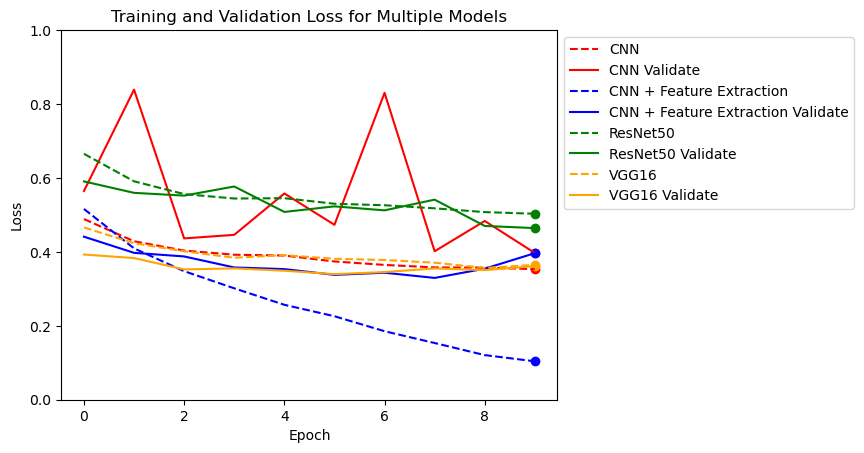
\includegraphics[scale=0.4]{LossEpochs.png}\newline
\end{figure}

The graph illustrates the trajectory of training and validation loss across the epochs for four distinct models (Figure 8). ResNet50 demonstrated overall the highest level of loss, both during training and validation phases, with only a modest reduction over time and minimal disparity between the training and validation losses. This suggests that while ResNet50 is capturing patterns within the data, its learning progress is sluggish and may benefit from optimization to enhance its learning rate. \newline
The standalone CNN model displayed a more favorable training loss curve, suggesting slow learning and improvement. However, the validation loss presented a more erratic pattern and was substantially higher, indicating that the model, despite its training efficacy, might be too attuned to the training data and not as adept at generalizing to unseen data. At some epochs the CNN validate loss was significantly higher than ResNet50. \newline
VGG16 maintained relatively favorable losses. Their validation losses were comparable to each other and remained close to the training losses, which is generally a positive sign. In fact, the VGG16 validate curve is slightly lower than its training curve. \newline
The CNN + feature extraction model displayed a rapid decline in training loss, suggesting efficient learning, and finished with the lowest training loss. However, the uptick in validation loss towards the end of the epochs hints at the onset of overfitting, although not as pronounced as with the standalone CNN model, since there was no drastic drop in validation error.

% Include packages in the preamble
\begin{table}[h]
\centering
\caption{Evaluation Metrics Comparison with Pham et al.}
\scriptsize
\setlength\tabcolsep{3pt} 
\begin{tabular}{|l|c|c|c|}
\hline
\makecell{\rotatebox{90}{\textbf{Evaluation Metric}}} & \makecell{\rotatebox{90}{\textbf{CNN + Feature Extr.}}} & \makecell{\rotatebox{90}{\textbf{Pham et al. Deep-CNN}}} & \makecell{\rotatebox{90}{\textbf{Pham et al. Derm. + Pract.}}} \\
\hline
Sensitivity & 0.88 & 0.85 & 0.74 \\ \hline
Specificity & 0.84 & 0.95 & 0.60 \\ \hline
AUC & 0.931 & 0.944 & 0.671 \\ \hline
\end{tabular}
\end{table}

A comparative evaluation of three distinct models – CNN + feature extractions, Pham et al. Deep-CNN, and Pham et al. with Dermatologists + Practitioners – is designed to provide valuable insights into the effectiveness and limitations of different approaches in medical diagnostic AI (Table 3). \newline \newline
For the CNN + feature extractions model using the HAM10000 dataset, it achieved a sensitivity of 0.88, specificity of 0.88, and an AUC of 0.931. Comparatively, Pham et al.'s model, applied to the ISIC 2019 dataset, showed a slightly lower sensitivity of 0.85 but a higher specificity of 0.95, along with a marginally better AUC of 0.944. The dermatologists’ results recorded were from Brinker et al where 100 skin lesion images were sent to 157 dermatologists in different German university hospitals \cite{pham2021ai} demonstrated a significantly lower sensitivity of 0.74 and specificity of 0.60, accompanied by a considerably lower AUC of 0.671.

\subsection{Discussion}
The CNN + feature extractions model, utilizing the HAM10000 dataset, demonstrated the commendable balance and overall performance compared to the VGG16, ResNet50, and CNN standalone model. It achieved an AUC of 0.931, a critical measure in medical diagnostics to mitigate the consequences of false diagnoses; where the cost of false negatives (missed diagnoses) and false positives (unnecessary treatments) can be significant. This model's superior specificity, slightly outdone by Pham et al.'s AUC of 0.944, may benefit from the diverse ISIC 2019 dataset, underscoring the influence of dataset selection on model efficacy. In the future, a more diverse dataset like ISIC 2019 can be used to expand and discover more capabilities of the hybrid CNN + feature extractions model. The involvement of dermatologists and practitioners in Pham et al.'s model resulted in all three metrics being compared, indicating human expertise from dermatologists and general practitioners underperformed. This outcome might reflect the challenges and limitations inherent in human evaluation, such as subjectivity or variability in judgment. These findings highlight the complexities and trade-offs in integrating human expertise with automated systems and stress the importance of leveraging the strengths of both approaches for improving diagnostic accuracy. \newline
The CNN + Feature Extraction model demonstrated high sensitivity, efficiently identifying true positives, likely due to the integration of additional informative features. This enhanced capability for detecting subtle indications of lesions, crucial in medical diagnostics, lead to a higher rate of false positives. Moreover, the model having the lowest specificity could be attributed to the model's heightened sensitivity to features associated with positive cases, potentially classifying ambiguous cases as positives to ensure no potential diagnoses are missed. \newline
Additional features in the CNN + feature extractions model likely contributed to its informed predictions. While its metrics were notably high, the fact that they seldom exceeded the 0.9 threshold—a benchmark indicative of exceptional performance as proposed earlier—signals room for improvement, potentially through architecture enhancements, more sophisticated feature engineering, or extended training. This threshold is critical, especially in high-stakes fields like medical diagnostics, where reliability is paramount. However, it's crucial to balance this pursuit of excellence with the practical requirements and context of the model's application, as the optimal performance criteria can vary significantly depending on the specific use case and the trade-offs between different types of errors. \newline
The standalone CNN model showed an ability to precisely identify negative cases, implied by its highest precision and specificity. While it is somewhat adept at ensuring what it classifies as positive is indeed positive, it tends to miss several actual positive cases due to its conservative approach, potentially due to its inability to detect less obvious features indicative of the positive class. The model's architecture, perhaps less complex than the others, might be highly tuned to specific features that define the negative class, thus leading to high specificity. Yet, this same focus might limit its ability to detect a broader range of characteristics that define positive cases, resulting in more false negatives. This behavior can be indicative of a model that's potentially overfitted to the negative class or not sufficiently capturing the diversity within the positive class, necessitating a more balanced or nuanced feature representation to improve recall without sacrificing precision and specificity. \newline
VGG16, characterized by its high sensitivity, effectively captured most true positives, as evidenced by its high recall, but also incurred numerous false positives. VGG16's performance likely stems from its deep architecture, which excels in extracting detailed features essential for complex image classification tasks, such as dermatological imaging. In discussion, VGG16's impressive results are likely owing to its deep learning architecture's ability to extract subtle and intricate features that are crucial for the classification of complex images, such as those found in dermatological imaging. \newline
ResNet50's notably lower recall suggests difficulties in identifying the positive class, which may stem from an array of issues such as insufficient training data, the need for additional epochs, or a more tailored learning strategy. Despite its depth and potential for complex feature learning, it may not have been able to adapt well to this dataset, possibly requiring more epochs, data, or a different learning strategy. Its structure, which is generally advantageous for learning hierarchical representations, may not have been fully leveraged due to insufficient training or the need for fine-tuning specific to the task at hand. \newline
Other models like standalone CNN and ResNet50 showed lower recall, indicating a struggle with correctly identifying true positives. This could be due to overfitting, inadequate learning of complex features, or a conservative prediction strategy, leading to more false negatives. That alongside the hybrid model’s performance generally implies these results highlight the trade-offs in machine learning model design, especially in medical applications where the balance between sensitivity and specificity is crucial. They also emphasize the importance of feature selection and model architecture, as seen in the improved performance of the CNN model with added feature extraction. \newline
In terms of metric evaluation, it can be debated that the recall/sensitivity metric is probably the least important. That metric can easily be changed by altering the threshold (the confidence percent for an image to be diagnosed positive). Reducing the threshold increases the recall as it allows more positive diagnosis (but can increase false positive rate). 
The main objective of the proposed work is to design a machine learning model that is able to accurately diagnose melanoma and benign moles. Considering the project's goal, the results indicate a relative success. CNN + Feature Extraction demonstrated promising capabilities in learning and generalization, as reflected in their training and validation performance metrics. However, the tendency towards overfitting in certain models underscores the need for careful balance between model complexity and generalization. The results also highlight the importance of model selection and tuning in accordance with the dataset's characteristics and the specific requirements of the task to ensure optimal performance. While no model achieved perfection, the observed trends and metrics suggest a strong foundation for further optimization and potential deployment in practical applications.

\section{Ethical Considerations}
The development of an AI model for medical diagnostics brings to the forefront a range of critical ethical considerations, particularly in the field of dermatology. One significant issue is the dataset’s failure to account for skin color variations. This oversight reflects a broader challenge in AI and ML: the need for inclusive datasets. The HAM 10000 dataset omits categorizing skin color, leading to potential biases in diagnostic outcomes. This lack of diversity in medical datasets is an ethical concern that underscores the importance of representing varied populations to ensure accuracy and fairness in medical diagnostics \cite{E;}. A Stanford University Project has stated 14/70 studies included at least 1 dataset with ethnicity descriptors. 7 out 70 included at least 1 dataset with skin tone descriptors \cite{Diverse}. This can lead to diagnostic models that are less accurate for individuals with skin tones as they are not as well represented in the data. This is known as sampling bias. In the future, the model should require or recommend diverse skin tones in images. For example, Adamson and Smith 2018 study in the “Journal of the American Academy of Dermatology” emphasized the importance of diversity in dermatological datasets as it provides more inclusive data to improve diagnostic accuracy across diverse populations. The dataset's lack of diversity in medical conditions is another point of concern, as it increases the risk of overfitting. Specifically, there were only 7 classes that were considered in the model. This can result in models that are overfitted to certain conditions and fail to recognize others, leading to disparities in diagnosis accuracy. In the future there should be an expansion of a dataset or look for more complex images. \newline \newline

Another big ethical consideration involves third-party apps in dermoscopy. These applications introduce ethical challenges such as data privacy and security, reliability, informed consent, and clinical validation. \newline

Moreover, the accessibility of the AI model poses significant ethical considerations, especially in terms of global equity. While the model can be integrated into mobile and computer applications, it does not guarantee universal access, particularly in under-resourced countries. This digital divide in AI technology access is a pressing ethical issue, highlighting the need to develop strategies to make these technologies more accessible and affordable worldwide. \newline

Furthermore, this work’s approach to setting diagnostic thresholds in the machine learning model missed substantially discussing the ethical implications of false positives and false negatives. These errors have serious consequences in medical diagnostics, with false positives potentially leading to unnecessary anxiety and procedures, and false negatives delaying critical treatment. It's critical to balance the model's sensitivity and specificity while scoring high, minimizing these risks while maintaining accurate diagnosis capabilities. According to the Nortar et al. (2018) study, false negatives are far worse than positives as they miss opportunities to save patients or help them. In the graph below, 0.7 was chosen as a threshold as it was before the slope had dropped. In terms of comparing the proposed model to others, there was a challenge as many of them did not include every metric used to evaluate the model. Furthermore, some models used a different dataset and trained with different classes. \newline

Going forward, this project will continue to enhance its framework and algorithms to boost the model's effectiveness. There is expected to be a plan in the future to implement more machine learning algorithms and techniques. One of them is unsupervised learning where all of the image labels aren’t given to the model. Instead, it must figure out what visual signs are a correlation to what class. This can be important as the model can help us inform better or figure out ways to educate dermatologists to train and detect what patterns have a significant impact. However, it could potentially be a risk for ethical considerations as it might have incorrect conclusions. Multi-class image classification would also be a good method to expand the ability of the proposed work as it can hopefully set a boundary between more classes than just melanoma and nevus. In fact, it can even be practiced very useful in diagnosing non-melanocytic lesions like basal cell carcinoma. 

\section{Replication Instructions}
\begin{enumerate}
    \item Anaconda Installation:

Start by downloading Anaconda from the official website:  \href{https://www.anaconda.com/download}{Free Download | Anaconda}. Make sure to select the version compatible with your operating system (Mac, Windows, Linux). It is important to note that Anaconda is a powerful suite of tools that simplifies package management and deployment for Python projects. Also, ensure there is at least 1.1GB of storage available for the installation.
\newline
    \item Anaconda Navigator Installation:
Once Anaconda is installed, open a terminal (for Linux/Mac) or Anaconda Prompt (for Windows). To install Anaconda Navigator, a graphical user interface that helps in managing conda packages, environments, and more, type the command:
\newline     
     conda install -c anaconda anaconda-navigator
\newline
    \item Launching Anaconda Navigator: Launch Anaconda Navigator from your computer's applications or by running the following command in the terminal/Anaconda Prompt:
\newline     
     anaconda-navigator
\newline
This tool streamlines access to different applications and tools for your data science projects.
\newline
    \item Jupyter Notebook: 
\newline
Inside Anaconda Navigator, launch Jupyter Notebook 6.5.4. Jupyter Notebook is chosen for its interactive features that facilitate live code, equations, visualizations, and explanatory text. Create a new Python 3 notebook, which allows for working with multiple code kernels and running different sections in an organized manner.
\newline
    \item Python Version:
\newline    
This project is using Python version 3.11.5, which is packaged by Anaconda, Inc. | (main, Sep 11 2023, 13:26:23) [MSC v.1916 64 bit (AMD64)].
\newline
    \item Dataset Download:
\newline   
Download the HAM10000 dataset. For example, you can download from \href{https://dataverse.harvard.edu/dataset.xhtml?persistentId=doi:10.7910/DVN/DBW86T}{[ViDIR Dataverse (harvard.edu)]}. Download both the images in the folder and the metadata in a .txt file format, which includes crucial information like image names and corresponding labels, vital for the classification system. This dataset is particularly chosen for its diversity and size, making it suitable for training a robust model.
\newline
    \item Python Packages: Make sure you have the necessary Python packages installed. You can install them using `conda` or `pip'.
    \begin{itemize}
        \item OpenCV (`cv2`): OpenCV library for computer vision tasks, used for image loading, color conversion, and Hu moments calculation.
        \item Pillow (`PIL`): Python Imaging Library (PIL) for working with images, used for opening and resizing images.
        \item NumPy (`numpy`): A fundamental package for numerical computing in Python, used for handling arrays and numerical operations.
        \item TensorFlow (`tensorflow`): An open-source deep learning framework developed by Google, used for building and training neural networks.
        \item Scikit-Learn (`sklearn`): A machine learning library for various tasks like data splitting, model evaluation, and metrics calculation.
        \item Matplotlib (`matplotlib`): A widely-used Python library for creating static, animated, and interactive visualizations in Python.
        \item Os: The `os` module provides functions for interacting with the operating system, used for working with file paths and directories.
        \item keras.layers: Keras layers for building the neural network architecture.
        \item keras.models: Keras models for defining and compiling the deep learning model.
        \item keras.optimizers: Keras optimizers for configuring the model's training optimization algorithm.
        \item keras.callbacks: Keras callbacks for monitoring and controlling the training process.
        \item keras.preprocessing.image: Keras tools for image preprocessing and data augmentation.
        \item sklearn.model\_selection.train\_test\_split: Used for splitting the dataset into training, validation, and test sets.
        \item sklearn.metrics: Various metrics for evaluating machine learning model performance, such as precision, recall, F1-score, ROC curve, AUC, and confusion matrix.
        \item ImageDataGenerator(from keras.preprocessing.image): Used for data augmentation, which helps improve the model's robustness.
    \end{itemize}

    \item File and Folder Organization:
\newline   
Organize your project files and folders according to the provided code architecture. It is crucial to correctly manage folder paths for images and labels and to meticulously handle the metadata, as it contains essential information for every image in the dataset.
     
\end{enumerate}

\section{Code Architecture Overview}
\subsection{Filtered Images}
\begin{figure}[h]
\caption{Filtered Images Diagram}
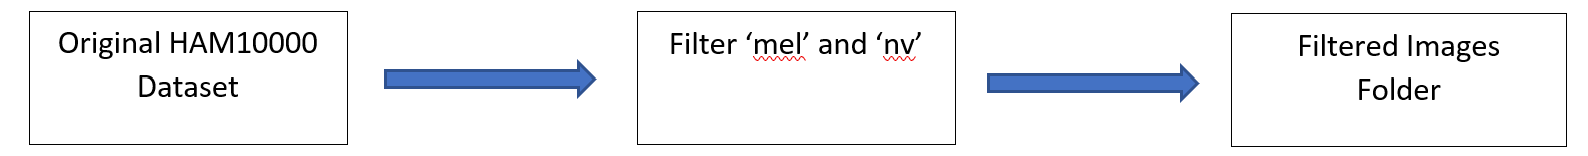
\includegraphics[scale=0.4]{Class Split.png}\newline
\end{figure}

SplitClasses is the initial step to organize the dataset, making it easier to handle during training and ensuring that each class is represented adequately (Figure 9).
It filters and segregates images into a new folder based on specific class labels—'mel' for melanoma and 'nv' for nevus. It begins by creating a target directory named `Filtered\_Images`, intended to store the selected subset of images. The script then parses a metadata file to create a dictionary (`labels\_dict`) that associates image IDs with their respective class labels.
\newline
The main operation occurs in a loop that iterates over all files in the `original\_folder`. During each iteration, the script checks if the current image's ID corresponds to one of the desired labels ('mel' or 'nv') in the `labels\_dict`. If there's a match, the image is deemed relevant and is copied to the `Filtered\_Images` folder. This ensures that only images of interest are included in the subsequent stages of data processing or model training.

\subsection{Image Resampling}
\begin{figure}[h]
\caption{Image Resampling Diagram}
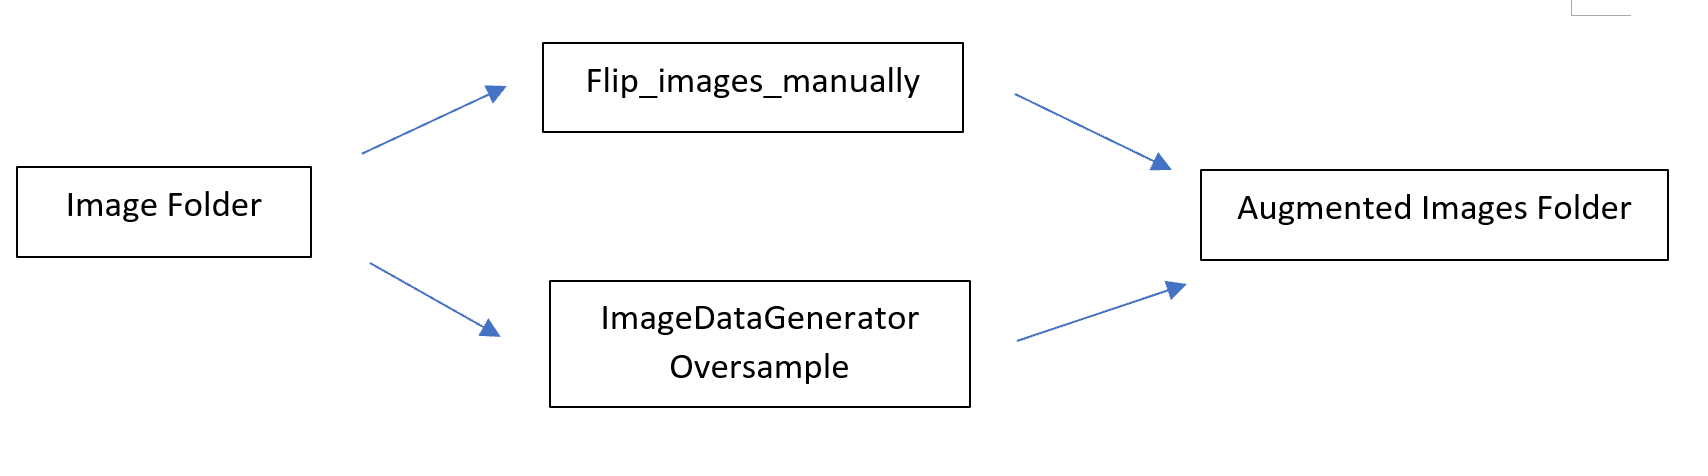
\includegraphics[scale=0.35]{Augment Images.png}\newline
\end{figure}

Image resampling follows, which increases the volume and diversity of the training data, especially important for classes with fewer samples (Figure 10).
\newline
The code initially sets up directories and reads image labels from the metadata as a txt file, creating a dictionary (`labels\_dict`) that maps image IDs to their respective labels, focusing on 'mel' and 'nv' classes. This dictionary serves as a filter to identify images.
\newline
The first part of the augmentation involves manual methods: `flip\_images\_manually` function is defined and executed to flip images horizontally, vertically, or both, for images labeled as 'mel'. These flipped images are then saved into an `augmented\_folder`, effectively increasing the dataset size with variations of existing images.
\newline
Next, the `ImageDataGenerator` from Keras is utilized to perform more complex duplications programmatically, such as random rotations, shifts, zooms, and flips. This tool applies specified transformations to each image in the dataset, simulating different perspectives and variations, further diversifying the dataset.
\newline
The code maintains a record of the augmented images by appending their paths to `augmented\_file\_path`, ensuring that the newly created dataset can be easily accessed for training purposes.
\newline
Finally, the `ImageDataGenerator` is also used in a loop to generate a certain number of images, as determined by a predefined threshold to balance the classes. These images are then added to the oversampled dataset, and their paths are appended to the metadata file.
\newline
The now completed and balanced dataset is then used by the model. 

\subsection{CNN Standalone}
\begin{figure}[h]
\caption{CNN Standalone Diagram}
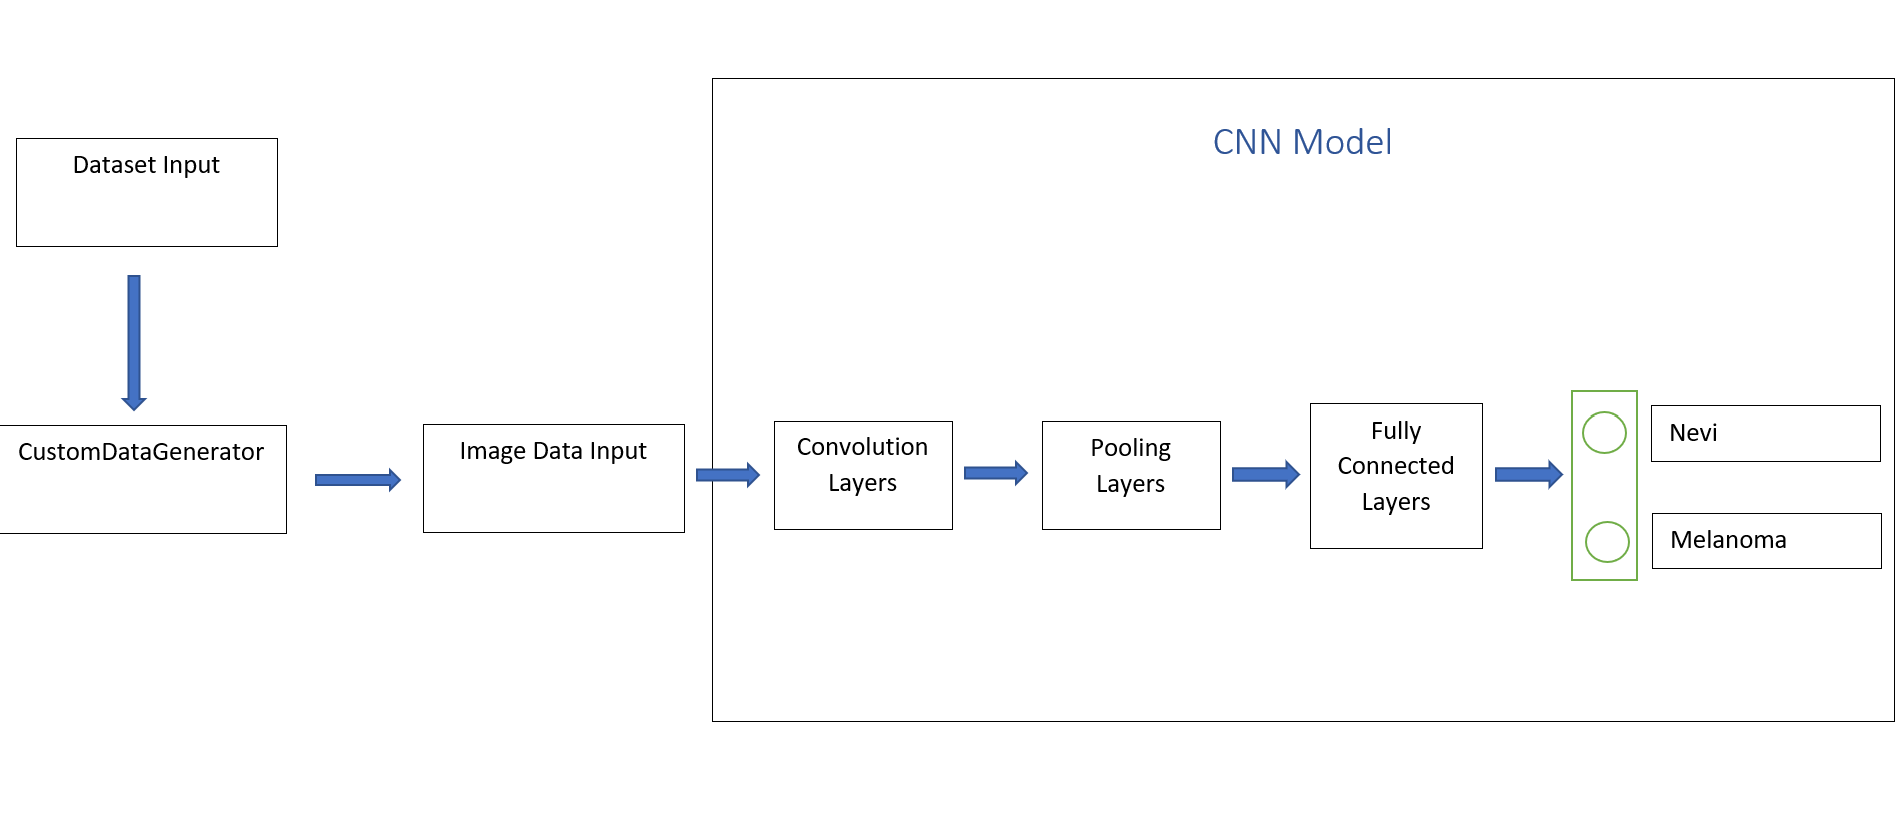
\includegraphics[scale=0.35]{CNN Model Architecture.png}\newline
\end{figure}

The CNN Model Architecture diagram represents a more traditional approach, where only image data is used as input (Figure 11).
\newline
It first sets up file paths for accessing the dataset, which comprises images pre-filtered to contain only 'mel' and 'nv' classes. A dictionary is created to map image filenames to their labels based on the metadata provided.
\newline
The core of the code is the `CustomDataGenerator`, which is designed to handle image loading, preprocessing, and augmentation, preparing the data for the model in batches. This class ensures data is fed in an efficient and manageable way during training.
\newline
The neural network itself is built using the Sequential API, layering convolutional blocks for feature extraction—which include convolution and max pooling layers—and dense layers for classification, all followed by batch normalization and activation functions to aid learning. The model is compiled with the Adam optimizer and binary cross entropy loss, suitable for the two-class problem at hand.
\newline
Training is executed with early stopping to prevent overfitting, and the model's performance is evaluated on a separate test set, with accuracy, precision, recall, and F1 scores reported. The results, including a confusion matrix, sensitivity, and specificity metrics, give a comprehensive overview of the model's classification abilities. Additionally, ROC and precision-recall curves are generated to assess the trade-offs between true positive rates and false positive rates at various threshold settings.


\subsection{CNN + Feature Extraction Model}
\begin{figure}[h]
\caption{CNN + Feature Extraction Diagram}
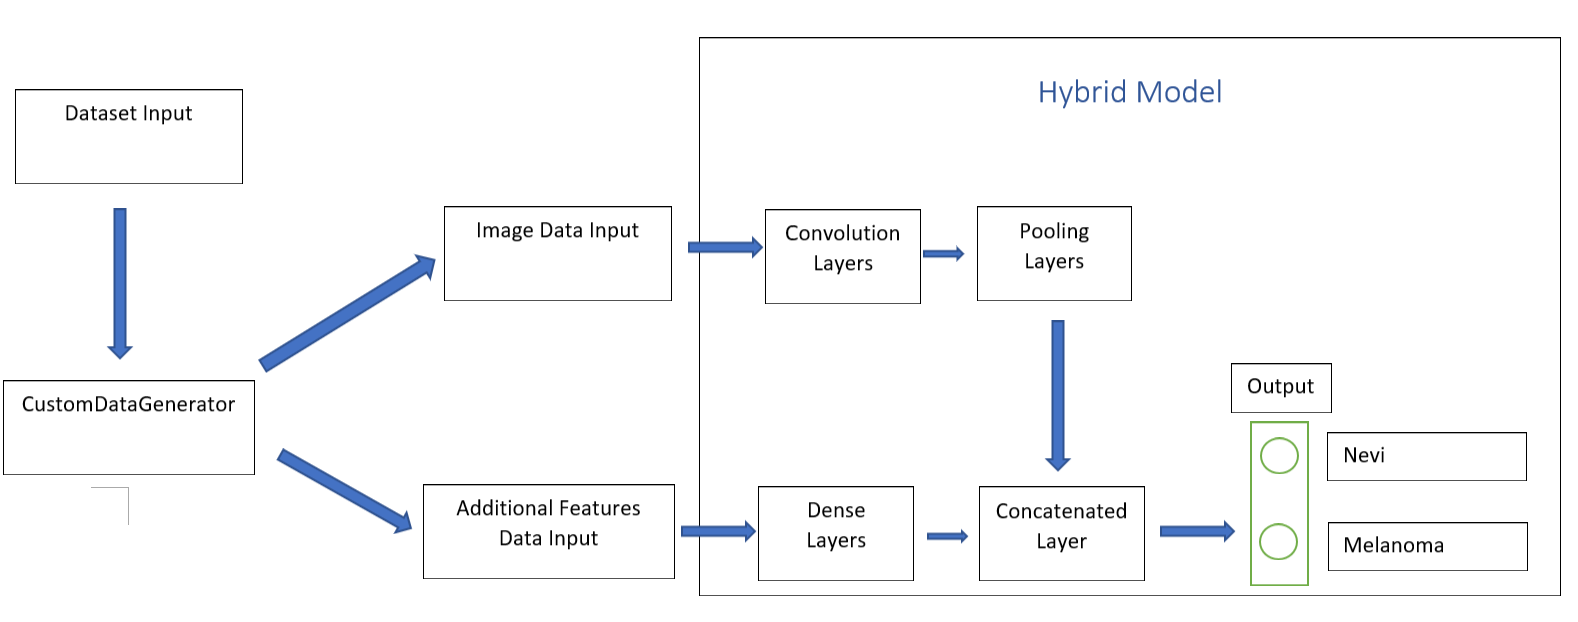
\includegraphics[scale=0.4]{Hybrid Model Architecture.png}\newline
\end{figure}
The Hybrid Model's code (CNN + Feature Extraction Model) architecture is designed for processing image data alongside additional extracted features to enhance predictive performance (Figure 12). Initially, image files are processed through a `CustomDataGenerator`, which resizes, normalizes, and optionally augments the images. Concurrently, image features are extracted using functions like `compute\_hu\_moments` and `compute\_color\_histogram`, and then combined with image data to form a unified input batch. The core model architecture employs convolutional layers for feature extraction from images, and dense layers for processing the additional features. These two streams are then merged into a concatenated layer, which feeds into a final output layer for binary classification—distinguishing between classes 'Nevus' and 'Melanoma'.
\newline
Training is executed with early stopping to prevent overfitting, and the model's performance is evaluated on a separate test set, with accuracy, precision, recall, and F1 scores reported. The results, including a confusion matrix, sensitivity, and specificity metrics, give a comprehensive overview of the model's classification abilities. Additionally, ROC and precision-recall curves are generated to assess the trade-offs between true positive rates and false positive rates at various threshold settings.
\newline
The model itself is defined with TensorFlow's Functional API, offering flexibility in combining diverse data inputs, which is critical for the hybrid approach. Sequential on the other hand, is unable to concurrently process diverse data types. 


\printbibliography

\end{document}
